%; whizzy section -pdf xpdf -latex ./whizzypdfptex.sh
% latex beamer presentation.
% platex, latex-beamer $B$G%3%s%Q%$%k$9$k$3$H$rA[Dj!%(B 

%     Tokyo Debian Meeting resources
%     Copyright (C) 2008 Junichi Uekawa

%     This program is free software; you can redistribute it and/or modify
%     it under the terms of the GNU General Public License as published by
%     the Free Software Foundation; either version 2 of the License, or
%     (at your option) any later version.

%     This program is distributed in the hope that it will be useful,
%     but WITHOUT ANY WARRANTY; without even the implied warranty of
%     MERCHANTABILITY or FITNESS FOR A PARTICULAR PURPOSE.  See the
%     GNU General Public License for more details.

%     You should have received a copy of the GNU General Public License
%     along with this program; if not, write to the Free Software
%     Foundation, Inc., 51 Franklin St, Fifth Floor, Boston, MA  02110-1301 USA

\documentclass[cjk,dvipdfm,12pt]{beamer}
\usetheme{Tokyo}
\usepackage{monthlypresentation}

%  preview (shell-command (concat "evince " (replace-regexp-in-string "tex$" "pdf"(buffer-file-name)) "&"))
%  presentation (shell-command (concat "xpdf -fullscreen " (replace-regexp-in-string "tex$" "pdf"(buffer-file-name)) "&"))

%http://www.naney.org/diki/dk/hyperref.html
%$BF|K\8l(BEUC$B7O4D6-$N;~(B
\AtBeginDvi{\special{pdf:tounicode EUC-UCS2}}
%$B%7%U%H(BJIS$B7O4D6-$N;~(B
%\AtBeginDvi{\special{pdf:tounicode 90ms-RKSJ-UCS2}}

\title{Debian Project and the Development Process, and how to co-work
with it.}
\subtitle{Cooperating with a large open source community}
\author{$B>e@n(B $B=c0l(B Junichi Uekawa\\dancer@debian.org\\IRC nick: dancerj}
\date{eeePC Developers' Conference 9 April 2008}
\logo{
\includegraphics[width=8cm]{image200607/openlogo-light.eps}}

\begin{document}

\frame{\titlepage{}}

% draft framework of talk.

\begin{frame}{}

This presentation is WIP.
\end{frame}

\begin{frame}{Junichi Uekawa}
\begin{itemize}
 \item Debian Developer since 2000
 \item Leading Debian JP Project since 2006
 \item Developer and maintainer of several Debian tools, such
       as pbuilder, dpatch, cowdancer, dsh, etc.
\end{itemize}
\end{frame}

\begin{frame}{What is Debian Project}
 \begin{itemize}%[<+->]
  \item 1 social contract, policy
  \item 11\footnote{etch official architectures} architectures 
  \item 209\footnote{as of 7 Jun 2007} mailing lists
  \item 1024\footnote{Jun 2007 developers who can vote}
	maintainers 
	\footnote{1939 if including 751 with packages, 
	1188 sponsored people,  \url{http://io.debian.net/~tar/bugstats/?dancer\%40debian.org}}
  \item 10223\footnote{etch official source package} packages
  \item All for Free Software.
 \end{itemize}
\end{frame}
% FIXME: update numbers with fresh new ones.

\begin{frame}{What is Debian Distribution}
\begin{itemize}
 \item Debian GNU/Linux (i386) and Debian GNU/Linux (amd64) being the
       most used product.
 \item many architectures
 \item many kernels: Linux, kFreeBSD, Hurd....
\end{itemize}
\end{frame}

\begin{frame}{Debian Communication framework}
 \begin{itemize}
  \item mailing lists and archives (lists.debian.org)
  \item IRC network (irc.debian.org)
  \item BTS (bugs.debian.org)
  \item Wiki (wiki.debian.org)
  \item svn, Git, ... (alioth.debian.org, svn.debian.org,
	git.debian.org, ...)
 \end{itemize}
\end{frame}

\begin{frame}{Debian Development Process}

\includegraphics[width=1\hsize]{image200805/develcycle.eps} 

All processes are package-centric

\end{frame}


\begin{frame}{User Process: Install / Upgrade}
 \begin{itemize}
  \item new package
  \item upgraded package
 \end{itemize}
\end{frame}

\begin{frame}{Tool: debconf}
\end{frame}

\begin{frame}{Tool: apt-listbugs}
\end{frame}

\begin{frame}{Tool: apt-listchanges}
\end{frame}

\begin{frame}{User Process: using package}

where to find documentation.
where to find more information.
reading the policy to know what is expected.

\end{frame}

\begin{frame}{User Process: Problem Report 1/2}
\begin{itemize}
 \item Sending patches.
 \item Sending reproducible problem.
 \item Sending vague feature requests.
\end{itemize}

What do you want to do today?
\end{frame}

\begin{frame}{User Process: Problem Report 2/2}
Tools to use 
\begin{itemize}
 \item gdb, strace, valgrind, oprofile, etc ... 
 \item http://bugs.debian.org/ with Mail Interface
\end{itemize} 
\end{frame}

\begin{frame}{Tool: Bugs.debian.org interface}
Tools to use 
\begin{itemize}
 \item Mail interface.
 \item Web interface.
 \item GUI tools.
\end{itemize} 
\end{frame}

\begin{frame}{Developer Process: upload}
 \begin{itemize}
  \item new package 
  \item new upstream
  \item bug handling 
 \end{itemize}
\end{frame}

\begin{frame}{Developer Process: bug receive}

\end{frame}

\begin{frame}{Developer Process: bug analyse}

\end{frame}


\begin{frame}{Developer Process: bug fix}

\end{frame}

\begin{frame}{Developer Process: package upload}

\end{frame}

\begin{frame}{localization}
 There are different localization aspects. Looking at translation at
 random gives:
\begin{itemize}
 \item po: upstream translation, shared with other distributions etc.
 \item po-debconf: debconf prompt translation.
 \item debian.org, webwml: web page translation
 \item DDTP: Description translation
 \item po4a: tool to support translation
\end{itemize}
\end{frame}

\begin{frame}{What's Next}
 \begin{itemize}
  \item Taipei Debian Community Kick off 
	-- Be part of the next movement
  \item 10 May 2008 (Sat)
 \end{itemize}
\end{frame}


\end{document}

;;; Local Variables: ***
;;; outline-regexp: "\\([ 	]*\\\\\\(documentstyle\\|documentclass\\|emtext\\|section\\|begin{frame}\\)\\*?[ 	]*[[{]\\|[]+\\)" ***
;;; End: ***
